\subsection{ROS 2 Middleware Implementations (RMW)}
\label{subsec:rmw}

\emph{ROS 2 middleware implementations} (RMW) merupakan implementasi dari sistem komunikasi \emph{middleware} yang ada pada ROS 2,
  menggantikan TCPROS/UDPROS yang ada pada ROS yang sebelumnya \citep{url:rmwdesign}.
Pada ROS 2, \emph{middleware} yang digunakan berbasis pada sistem yang dimiliki oleh DDS,
  dimana DDS sendiri memiliki berbagai macam implementasi seperti RTI Connext DDS \citep{url:rmwdesign} eProsima Fast DDS \citep{url:fastdds},
  Eclipse Cyclone DDS \citep{url:cyclonedds},
  dan lain sebagainya.

\begin{figure}[ht]
  \centering
  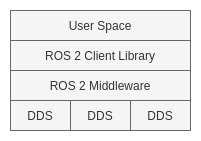
\includegraphics[scale=0.55]{gambar/layer-sistem-ros2.png}
  \caption{\emph{System layer} yang ada pada ROS 2 \citep{url:rmwdesign}.}
  \label{fig:layersistemros2}
\end{figure}

Seperti yang terlihat pada gambar \ref{fig:layersistemros2},
  \emph{system layer} yang ada pada ROS 2 terdiri atas \emph{user space} di bagian paling atas,
  kemudian \emph{ROS 2 client library} (RCL), RMW, dan terakhir DDS.
Di sini, peran RMW adalah sebagai penghubung antara RCL dengan implementasi DDS yang digunakan.
Saat ini ROS 2 sudah mendukung beberapa implementasi DDS yang bisa digunakan dalam bentuk \emph{ROS 2 package},
  seperti pada \emph{package} \lstinline{rmw_connextdds} yang digunakan untuk menjalankan implementasi DDS dari RTI Connext DDS,
  \emph{package} \lstinline{rmw_fastrtps} yang digunakan untuk menjalankan implementasi DDS dari eProsima Fast DDS,
  dan lain sebagainya.
